\documentclass[sigconf,authorversion,review,authordraft]{webmedia}
\acmDOI{10.5753/webmedia_estendido.2025.16796}

% -- basic config
\usepackage{array} % support p{width}
\usepackage{tabularx} % flexible column X
\usepackage{booktabs} % \toprule, \midrule, \bottomrule
\usepackage{listings} % code listing
\usepackage{subcaption} % subfigures
\usepackage{ragged2e} % \justify
\usepackage{graphicx} % includegraphics
\usepackage{acronym} % \newacro and \ac
\usepackage{lipsum}
\usepackage{url} % \url
\newcommand{\ie}[0]{\textit{i.e.},~}
\newcommand{\eg}[0]{\textit{e.g.},~}
\newcommand{\etal}[0]{\textit{et al.}~}

% -- basic tikz
\usepackage{tikz}
\usetikzlibrary{arrows.meta, positioning, shapes, fit}

% -- others
\newacro{CNN}{Convolutional Neural Network}
\newacro{RNN}{Recurrent Neural Network}
\newacro{LLM}{Large Language Model}
\newacro{GAN}{Generative Adversarial Network}
\newacro{CV}{Computer Vision}
\newacro{ML}{Machine Learning}
\newacro{AI}{Artificial Intelligence}

\AtBeginDocument{%
  \providecommand\BibTeX{{%
    \normalfont B\kern-0.5em{\scshape i\kern-0.25em b}\kern-0.8em\TeX}}}
\settopmatter{printacmref=false, printfolios=false}

\setevent{wtvdi}
\proceedingsDetails[WTVDI’2025]{VIII Workshop Futuro da TV Digital Interativa (WTVDI 2025). Anais Estendidos do XXXI Simpósio Brasileiro de Sistemas Multimídia e Web}{2025}{Rio de Janeiro/RJ, Brasil}
\ISSN{2596-1683}

%%%%%%%%%%%%%%%%%%%%
\begin{document}
%%%%%%%%%%%%%%%%%%%%

\title{Artificial Intelligence Applications in TV Industry Workflow}
\author{Alan L. V. Guedes}
\email{a.guedes@reading.ac.uk}
\orcid{0000-0003-0110-9975}
\affiliation{%
  \institution{University of Reading}
  \city{Reading}
  \country{UK}
}
\renewcommand{\shortauthors}{Guedes, A.L.G.}
\begin{abstract}
  The TV industry is going through a major change due consumers need for high-quality, diverse, and customized content. This leads to increase production costs while the  production time shrink. To deal with these challenges, the industry is levering the use of Artificial Intelligence to improve and optimize their processes. This paper gives a summary of how it is being used in existing literature and publicly available use cases. But different than other works, we put them application in perspective of the TV Industry workflow of pre-production, production, post-production, and distribution.
\end{abstract}
\keywords{TV Industry, Artificial Intelligence, TV production}
\maketitle

%%%%%%%%%%%%%%%%%%%%
\section{Introduction}
\label{sec:introduction}
%%%%%%%%%%%%%%%%%%%%

The TV industry is undergoing a major transformation due to the rapid advancement of digital technologies and the changing preferences of audiences. The demand for high-quality, diverse, and personalized content is increasing, while production costs and timelines are decreasing. To address these challenges, the TV industry is leveraging \ac{AI} to automate repetitive workflows, improve visual quality, and enhance audience retention and experience. This usage still growing inside the industry, which lack better clarity and application scenarios. For instance, according to a study by the IBC (International Broadcasting Convention) 2017, the use of \ac{AI} in broadcast and media is still at an early stage, with only 8\% of media technology buyers having used it before\footnote{\url{https://theiabm.org/ai-broadcast-media-snapshot}}.

This paper provides an overview of current \ac{AI} applications in the TV industry, based on existing literature and publicly available use cases. As illustrated in \autoref{fig:pipeline}, we organize these applications according to the television workflow defined by Owens \cite{owens2023}: \textbf{pre-production}, \textbf{production}, \textbf{post-production}, and \textbf{distribution}. In each phase, \ac{AI} reshapes or optimize some step from planning and creative ideation in pre-production, to enhancing and synthesizing media assets in post-production. This workflow perspective emphasizes how \ac{AI} is not confined to a single phase. Also, as we seen further, its applications flourish first on the post-production and distribution but now are present in the entire TV workflow.

\begin{figure}[ht!]
  \centering
  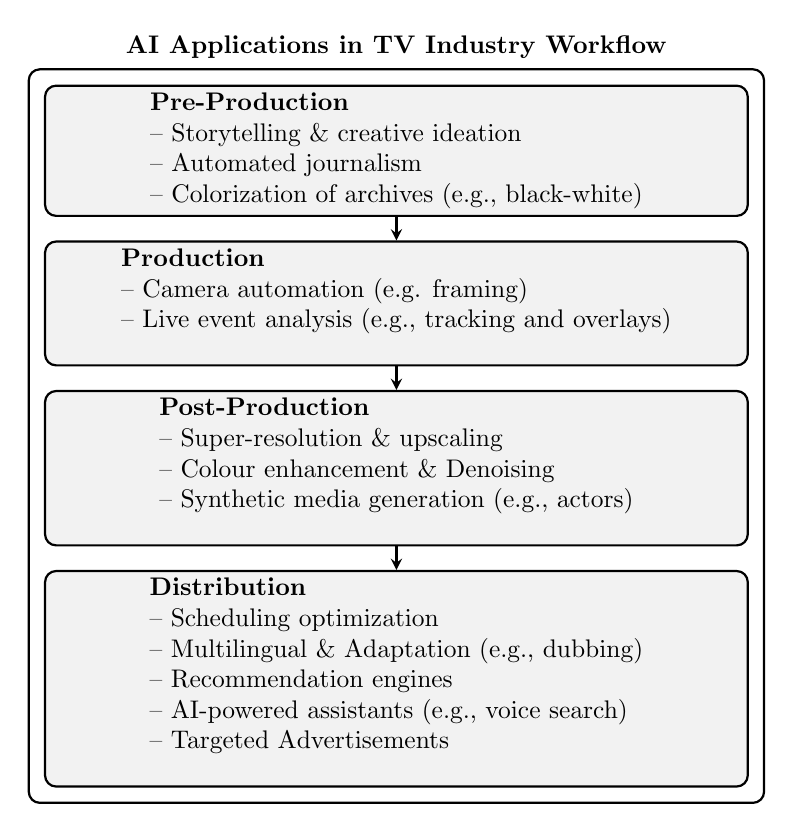
\begin{tikzpicture}[node distance=3mm,>=stealth,thick,scale=0.92, every node/.style={scale=0.92}]
    \tikzstyle{stage}=[rectangle, rounded corners, draw, align=flush left, minimum width=0.8\linewidth, inner sep=1mm]
    % Workflow nodes
    \node[stage, fill=gray!10] (pre) {\textbf{Pre-Production}\\
      -- Storytelling \& creative ideation\\
      -- Automated journalism \\
      -- Colorization of archives (e.g., black-white)
    };
    \node[stage, fill=gray!10, below=of pre] (prod) {\textbf{Production}\\
      -- Camera automation (e.g. framing)\\
      -- Live event analysis (e.g., tracking and overlays)\\
    };
    \node[stage, fill=gray!10, below=of prod] (post) {\textbf{Post-Production}\\
      -- Super-resolution \& upscaling\\
      -- Colour enhancement \& Denoising\\
      -- Synthetic media generation (e.g., actors)\\
    };
    \node[stage, fill=gray!10, below=of post] (dist) {\textbf{Distribution}\\
      -- Scheduling optimization\\
      -- Multilingual \& Adaptation (e.g., dubbing)\\
      -- Recommendation engines\\
      -- AI-powered assistants (e.g., voice search)\\
      -- Targeted Advertisements\\
    };
    % Arrows between stages
    \draw[->] (pre.south) -- (prod.north);
    \draw[->] (prod.south) -- (post.north);
    \draw[->] (post.south) -- (dist.north);
    % Big surrounding box
    \node[draw, thick, rounded corners, fit=(pre)(prod)(post)(dist), inner sep=6mm, label={\textbf{AI Applications in TV Industry Workflow}}] {};
  \end{tikzpicture}
  \caption{AI applications in the perspective of the TV Industry workflow \cite{owens2023}.}
  \Description{}
  \label{fig:pipeline}
\end{figure}

The remainder of the paper is organized as follows. Section~\ref{sec:related-work} presents related work. Next four sections list the AI applications in each of TV workflow phase (Sections~\ref{sec:pre-production}, \ref{sec:production}, \ref{sec:post-production} and \ref{sec:distribution}). Finally, Section~\ref{sec:final-remarks} offers final remarks and discusses challenges.

%%%%%%%%%%%%%%%%%%%%
\section{Related Work}
\label{sec:related-work}
%%%%%%%%%%%%%%%%%%%%

Some previous works share our goal and offering an overview of AI in TV and media industry. Caramiaux \etal\cite{amato2019ai} and Anantrasirichai \etal\cite{anantrasirichai2022artificial} are more general and focus on the media industry. While Santos \etal\cite{journalmedia3010002} specifically targets journalism, and Connock \etal\cite{connock2024} targets TV but only in UK.

Caramiaux \etal\cite{amato2019ai} provide an overview of the impact of \ac{AI} in the media and creative industries, highlighting its transformative role across sectors such as music, images and visual art, content and narration, and information and media. The paper discusses the challenges and potential of AI in enhancing creativity, production, and consumption, while also addressing societal and technological hurdles. It emphasizes the need for interdisciplinary collaboration to fully harness AI's capabilities in creative processes and underscores the importance of inclusivity and diversity in the development of AI-driven creative tools. Additionally, it explores the implications of AI on personalization, open society, and the creative economy, suggesting a future where AI contributes significantly to research and development in the media and creative sectors.

Anantrasirichai \etal\cite{anantrasirichai2022artificial} provide a review of \ac{AI} technologies and their applications within the creative industries. They cover a range of AI methodologies and categorize applications into algorithms like \ac{CNN}, \ac{GAN}, \ac{RNN}, and other. They conclude that AI benefit in creative industries lies in augmenting human creativity rather than replacing it. Connock \etal\cite{connock2024} describe the role of \ac{AI} in British television from extensive interviews. It highlights how AI has progressively influenced all stages of the TV Industry workflow. Connock argues that AI first moving into creative development with generative tools, synthetic media, and agent-based models. The work situates these technological shifts within the broader challenges facing the TV industry, including global competition, funding pressures, and copyright risks, suggesting that AI could simultaneously disrupt and reinvigorate British television's creative and commercial future.

Santos \etal\cite{journalmedia3010002} discuss and analyse how AI technologies are being developed within journalism and present an agenda for future research. They highlight that while \ac{AI} has the potential to aid the news industry, most \ac{AI} news projects are funded by tech companies, which limits the scope to a few players. The paper also addresses challenges faced by newsrooms, including resistance to change and lack of skills, which can delay technological innovations.

Previous work from us \cite{guedes2020future} discusses future usage scenarios in the context of Edge AI, where \ac{ML} models run on TV devices. However, that work does not provide the view offered in this current survey.

\label{sec:pre-production}

%%%%%%%%%%%%%%%%%%%%
\section{Pre-Production}
%%%%%%%%%%%%%%%%%%%%
Pre-production defines the creative and preparation for create TV content. For instance, build journalistic material or prepare the programme story.

\textbf{Automated journalism.} Automated journalism is now widely used. For example, the BBC reported on the UK general election in 2019 using such tools.\footnote{\href{https://www.bbc.com/news/technology-50779761}{https://www.bbc.com/news/technology-50779761}} Forbes uses an AI-based content management system called Bertie to assist reporters with first drafts and templates for news stories.\footnote{\url{https://www.forbes.com/sites/nicolemartin1/2019/02/08/did-a-robot-write-this-how-ai-is-impacting-journalism/\#5292ab617795}} The Washington Post also has a robot reporting program called Heliograf.\footnote{\url{https://www.washingtonpost.com/pr/wp/2016/10/19/the-washington-post-uses-artificial-intelligence-to-cover-nearly-500-races-on-election-day}} In 2020, Microsoft announced the use of automated systems to select news stories for the MSN website.\footnote{\url{https://www.bbc.com/news/world-us-canada-52860247}} These applications demonstrate that current AI technologies can support human journalists in constrained cases, increasing production efficiency. Kaneko \etal\cite{kaneko2020ai} discuss how NHK has developed a new AI-driven broadcasting technology called
\textit{Smart Production}, which extracts events and incidents from diverse sources such as social media feeds (e.g., Twitter/X), local government data, and interviews, integrating them into a human-friendly, accessible format.

\textbf{Storytelling \& creative ideation.} Narrative is fundamental to all forms of creativity across art, fiction, journalism, gaming, and other entertainment. \ac{ML} has been used both to create stories and to optimize the use of supporting data, for example, organizing and searching through large archives for documentaries. In 2016, an IBM model\footnote{\url{https://www.ibm.com/blogs/think/2016/08/cognitive-movie-trailer}} composed a 6-minute movie trailer for the horror film "Morgan" by training on more than 100 trailers of horror films, enabling it to learn normative structure and patterns. Ross Goodwin\footnote{\url{https://bigcloud.global/filming-the-future-how-ai-was-a-director-for-a-sci-fi-short}} proposed the model Benjamin, which uses NLP and Markov chain algorithms for scriptwriting. Benjamin's capabilities were showcased in three movies: "Sunspring" (2016), written by feeding the \ac{AI} hundreds of sci-fi scripts; "It's No Game" (2017), which featured AI-generated dialogue; and "Zone Out" (2018), where Benjamin utilized facial swapping technology and voice generators to integrate actors' performances with scenes from public domain films.

More recently in 2024, Mirowski \etal\cite{mirowski2023co} proposed "Dramatron" a system that uses \ac{LLM} to generate scripts and screenplays hierarchically. Figure \ref{fig:dramaton} show hierarchical story generation approach to create coherent long-form scripts by structuring the generation process into layers, starting from a log line to develop titles, characters, plots, and dialogues. The system also supports a co-creative process by including industry professionals to co-write scripts with Dramatron, providing feedback that led to system improvements. The scripts were later staged at a theatre festival, and an expert evaluation was performed with professionals from the theatre and film industry to assess Dramatron's usability and creative output.

\begin{figure}[!ht]
  \centering
  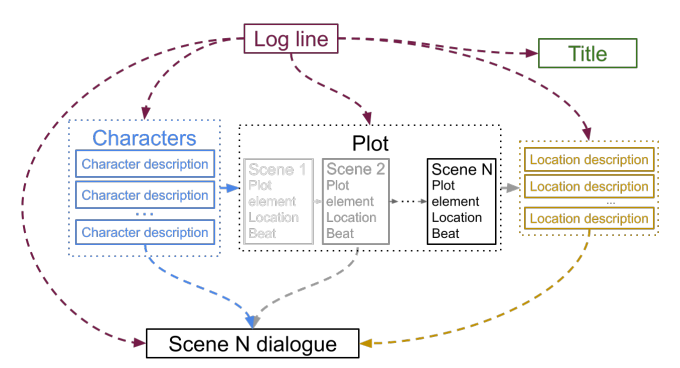
\includegraphics[width=0.8\linewidth]{assets/image7.png}
  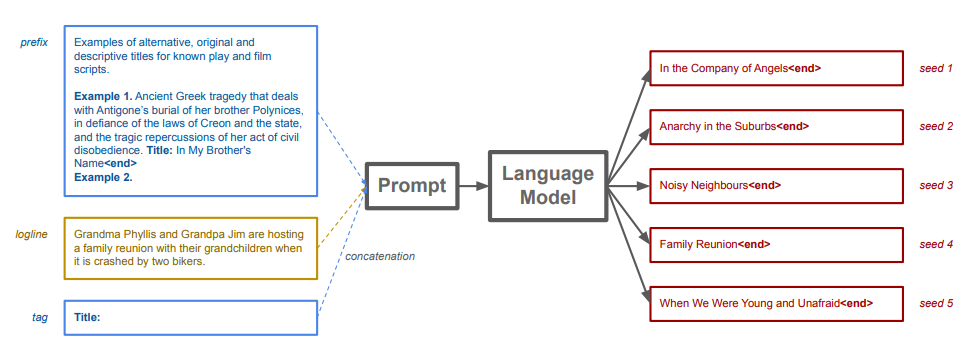
\includegraphics[width=\linewidth]{assets/image8.png}
  \caption{Dramaton hierarchical story generation and LLM prompting. }
  \Description{}
  \label{fig:dramaton}
\end{figure}

%%%%%%%%%%%%%%%%%%%%
\section{Production}
\label{sec:production}
%%%%%%%%%%%%%%%%%%%%
In the production, AI has been most visible when drive robotic cameras, automatically framing shots or in live broadcasting.

\textbf{Camera Automation.}
Camera automation leverages  \ac{CV} and deep learning models to support framing, tracking, and replay selection in live production. Convolutional neural networks (CNNs) are particularly effective for object detection and motion tracking, enabling automated shot composition in sports and event broadcasting \cite{anantrasirichai2022artificial}. These systems reduce the operational burden on camera operators and enhance consistency in fast-paced environments. Nevertheless, human oversight remains essential to ensure that automated decisions respect editorial standards and creative intent \cite{wright2023ai,kaneko2020ai}.

\begin{figure}[!ht]
  \centering
  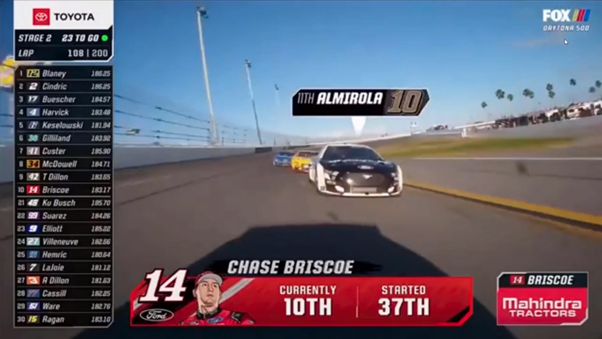
\includegraphics[width=0.8\linewidth]{assets/image1.png}
  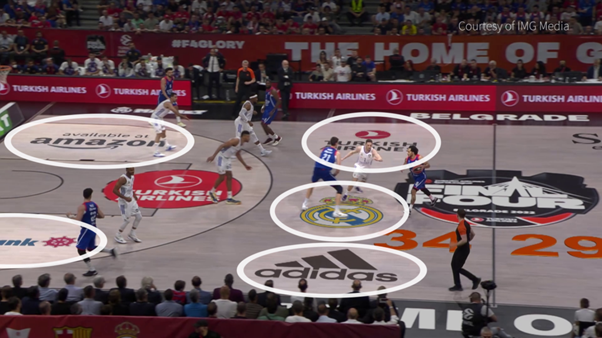
\includegraphics[width=0.8\linewidth]{assets/image2.png}
  \caption{Virzrt visual analysis of live sports events. }
  \Description{}
  \label{fig:live}
\end{figure}

\textbf{Live Event Analysis.} In sports and live entertainment, tracking, analytics, and predictive insights power data-driven commentary and augmented reality (AR) overlays. ML processes large quantities of data and efficiently extracts key statistics, patterns, and—most importantly—real-time predictions of plays, matches, results, and more. With faster, more relevant, and insightful data, broadcasters can bring validated insights into the game and add to their arsenal of tools in the constant battle for audience attention. Efficient visualization tools and connected AR systems enable better gameplay insight, from play forecasts to deep statistical backgrounds. By transferring analysis to the screen, producers and broadcasters enrich the viewing experience for both first- and second-screen audiences. Extracted data from ML can be combined with high-end analytics software to deliver automated analyses of plays, which can be offered to producers as needed. Additionally, this data can drive higher engagement and quality in hands-on productions. For example, Formula 1 partnered with Amazon Web Services (AWS)\footnote{\url{https://aws.amazon.com/blogs/architecture/formula-1-using-amazon-sagemaker-to-deliver-real-time-insights-to-fans-live}} to leverage ML for analysis of over 65 years of race data, as well as dozens of live data points, to offer audiences mid-race breakdowns and predictions about the action on screen. Wright \etal\cite{wright2023ai} present how the BBC created a proof-of-concept system for automated coverage of live events, where an AI-based system performs shot framing (wide, mid, and close-up shots), sequencing, and shot selection automatically. However, initial results show that the algorithm still needs improvement before it can replace human operators.

During the 2022 World Cup in Qatar, 12 dedicated tracking cameras were mounted under the roof of the stadium to track each player. ML methods were used to detect the exact relative positions on the pitch in real time. The ball also contained inertial sensors, the data from which could be combined and used to assess offside calls. The company Vizrt\footnote{\url{https://www.vizrt.com/community/blog/5-ways-artificial-intelligence-and-machine-learning-will-make-sports-TVing-smarter}} describes its vision of how object tracking can improve live events. Object identification within video frames can be used for virtual advertising and enhancing fan engagement. Enhanced scene understanding \ac{AI} improves live sports broadcasting by enabling automated keying, which allows for real-time graphic insertions into live streams. This results in quick setup times and continuous adjustment, enhancing the viewing experience, illustrate in Fig. \ref{fig:live}. Advancements in \ac{AI} and \ac{ML} also allow for real-time content and graphic decisions during live broadcasts, including inserting and replacing objects in the stream, providing viewers with an enriched and engaging experience.

%%%%%%%%%%%%%%%%%%%%
\section{Post-Production}
\label{sec:post-production}
%%%%%%%%%%%%%%%%%%%%

\begin{figure}[!ht]
  \centering
  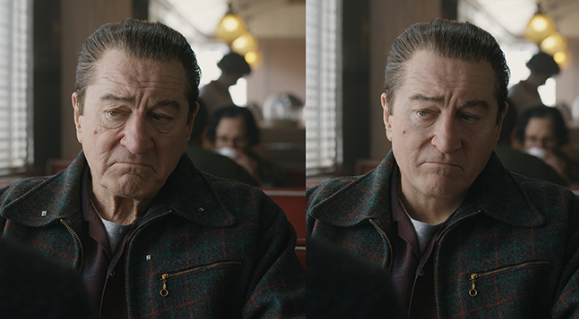
\includegraphics[width=0.9\linewidth]{assets/image9.png}
  \caption{AI-powered VFX helped de-age actor in "The Irishman".}
  \Description{}
  \label{fig:irishman}
\end{figure}

\begin{figure}[!ht]
  \centering
  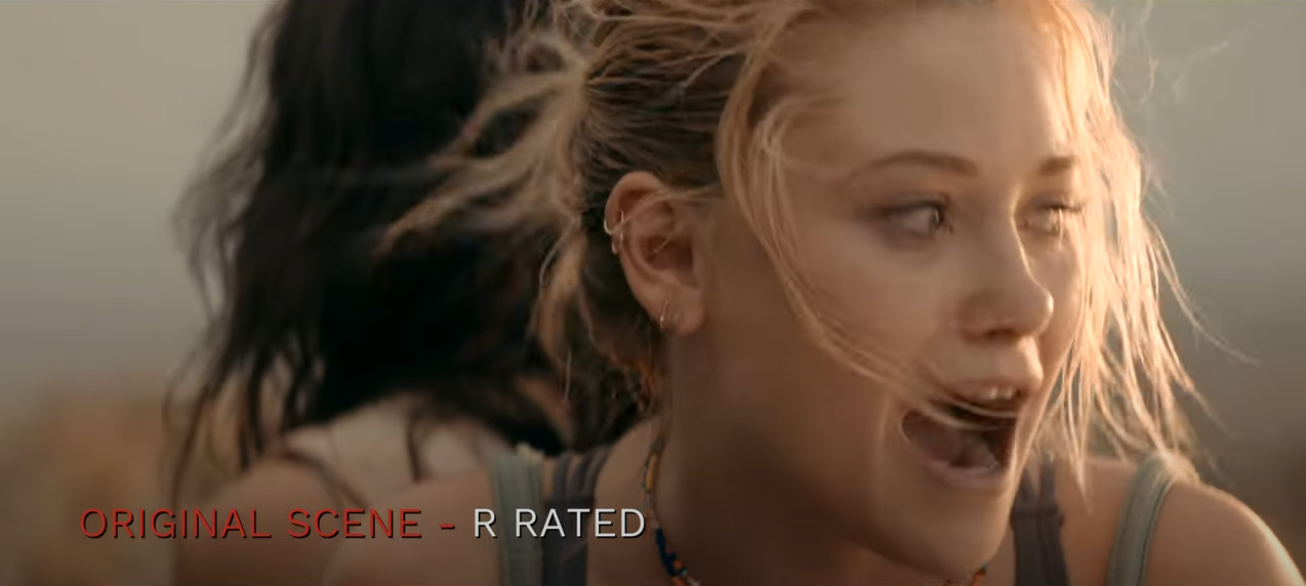
\includegraphics[width=0.7\linewidth]{assets/image3.png}
  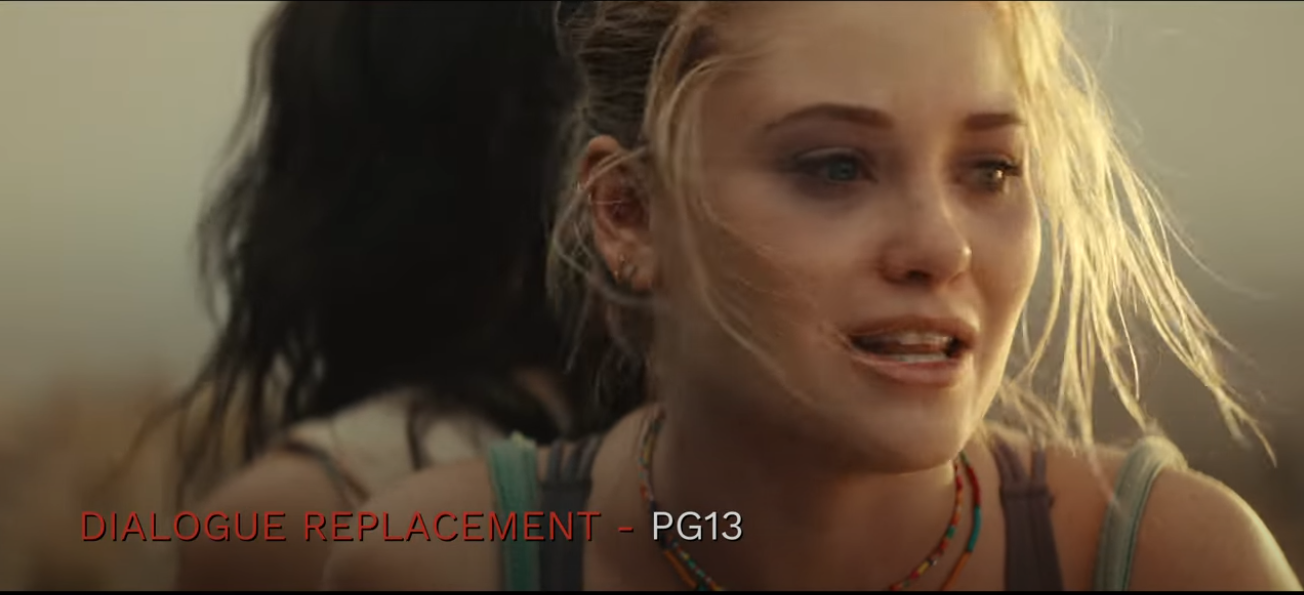
\includegraphics[width=0.7\linewidth]{assets/image4.png}
  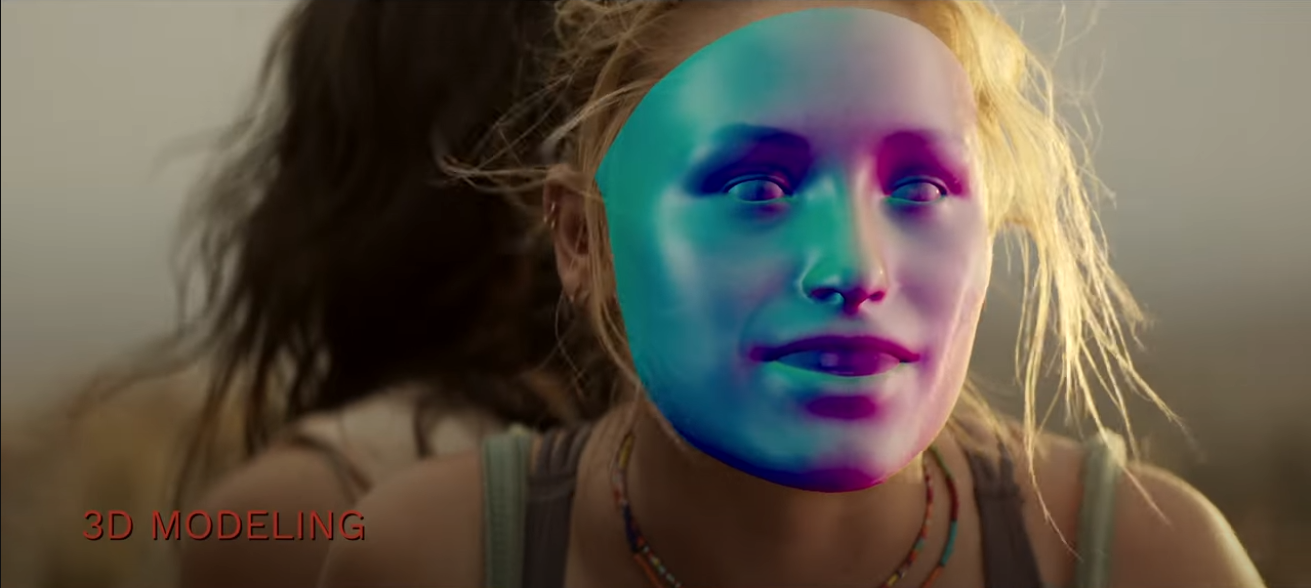
\includegraphics[width=0.7\linewidth]{assets/image5.png}
  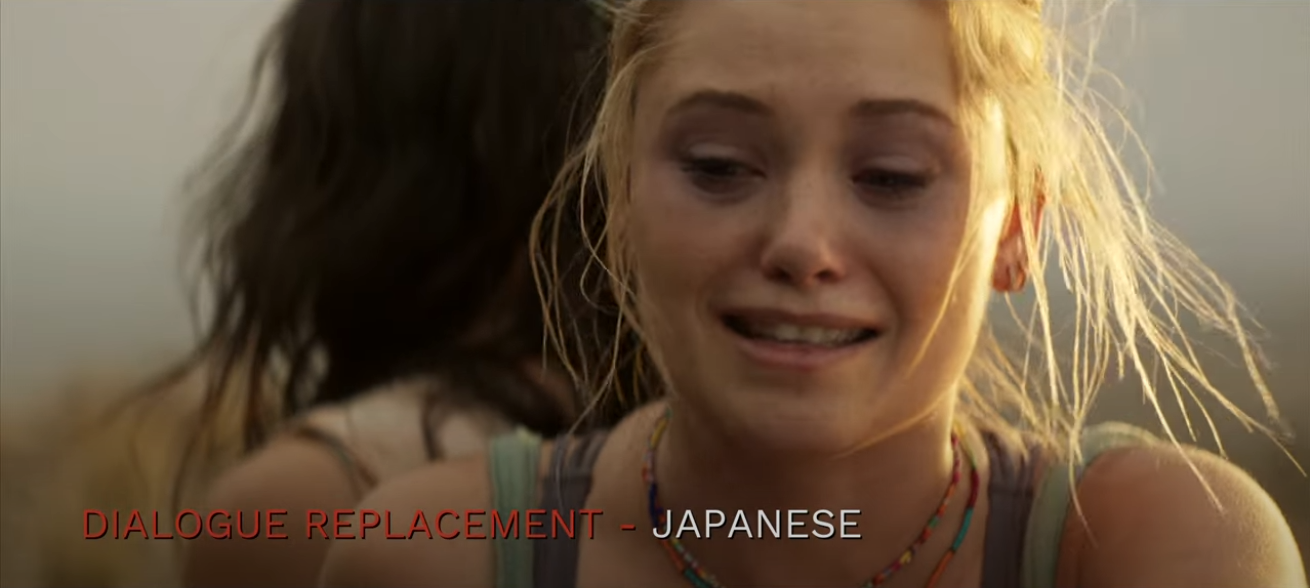
\includegraphics[width=0.7\linewidth]{assets/image6.png}
  \caption{Flawless TrueSync on the movie "Fall" for PG13 and multilingual adaptation.}
  \Description{}
  \label{fig:truesync}
\end{figure}

Post-production has seen significant experimentation with machine learning, particularly in image enhancement and synthetic content generation.

\textbf{Super-Resolution \& Upscaling.}
Restoration from SD or HD to UHD/8K with temporal models recovers detail and prepares catalogues for modern displays. Super-resolution (SR) approaches have gained popularity in recent years\cite{he2023comparative}, enabling the up sampling of images and video both spatially and temporally. This is useful for up-converting legacy content for compatibility with modern formats and displays. SR methods increase the resolution (or sample rate) of a low-resolution (LR) image or video. In the case of video sequences, successive frames can be used to construct a single high-resolution (HR) frame. Although the basic concept of SR algorithms is simple, there are many challenges related to perceptual quality and limited available data. For example, LR video may be aliased and exhibit sub-pixel shifts between frames, so some points in the HR frame do not correspond to any information from the LR frames. When applied to video sequences, super-resolution methods can exploit temporal correlations across frames as well as local spatial correlations within them. Pixop, France TV Lab, and Harmonic Inc\footnote{\url{https://www.pixop.com/blog/super-resolution-in-broadcasting}} conducted an experiment using Pixop's Deep Restoration and Super Resolution filters to upscale SD content to UHD 4K, achieving better results than traditional methods.

\textbf{Colorization of Archives} AI colorization, cleanup, and metadata enrichment prepare legacy assets before recording, ensuring consistency in art direction and technical readiness.
This can be useful for colouring archival black-and-white content, enhancing infrared imagery (e.g., in low-light natural history filming), and restoring the colour of aged film. The first AI-based techniques for colorization used a CNN with only three convolutional layers to convert a grayscale image into chrominance values, then encoder-decoder networks are employed in Xu \etal\cite{xu2020stylization}. A good example is the film "They Shall Not Grow Old" (2018) by Peter Jackson, which colorized (and corrected for speed and jerkiness, added sound, and converted to 3D) 90 minutes of footage from World War One. The workflow was based on extensive studies of WW1 equipment and uniforms as a reference point and involved time-consuming use of post-production tools.

\textbf{Colour Enhancement \& Denoising} AI-assisted grading and look transfer standardize palettes across sequences. The human visual system employs many opponent processes, both in the retina and visual cortex, which rely heavily on differences in colour, luminance, or motion to trigger salient reactions. Contrast is the difference in luminance and colour that makes an object distinguishable and is an important factor in subjective evaluation of image quality. Low-contrast images exhibit a narrow range of tones and can appear flat or dull. Modern methods have further improved performance by exploiting autoencoders and residual learning\cite{lore2017llnet}.

Noise and compression artifacts are reduced to improve perceived quality and coding efficiency. Noise can be introduced from various sources during signal acquisition, recording, and processing, and is often attributed to sensor limitations under extreme conditions. It is characterized as additive, multiplicative, impulsive, or signal-dependent, and by its statistical properties. Noise is not only visually distracting, but can also affect the performance of detection, classification, and tracking tools. Denoising nodes are therefore commonplace in post-production workflows, especially for challenging low-light natural history content\cite{anantrasirichai2020encoding}. In addition, noise can reduce the efficiency of video compression algorithms, since the encoder allocates wasted bits to represent noise rather than signal, especially at low compression levels. This is why film-grain noise suppression tools are employed in certain modern video codecs (such as AV1) prior to encoding. With AI-powered denoising, creators can remove grain from their renders and create noise-free, interactive images in real time.

\textbf{Synthetic Media Generation.}
Generative models, such as generative adversarial networks (GANs), are increasingly applied in television for the creation of trailers, highlight reels, and promotional content. By learning audiovisual patterns, these models can synthesize realistic sequences that complement or expand existing material \cite{amato2019ai}. In the creative industries, synthetic humans and AI-driven voice synthesis are already being tested, providing cost-effective production options while raising important questions around copyright and authenticity \cite{anantrasirichai2022artificial}. These tools open new opportunities for storytelling but must be deployed transparently to preserve audience trust.

\textbf{Multilingual \& Adaptation.}
AI-driven dubbing and subtitling are transforming the global distribution of audiovisual content. AI-based translation (NMT) and speech synthesis systems now allow broadcasters to deliver real-time or near-real-time multilingual versions of programs, significantly reducing turnaround times \cite{journalmedia3010002}. This has proven especially valuable in high-volume domains such as news and sports, where speed and accessibility are paramount. Recent innovations also include AI-powered lip-synchronization technologies, such as Flawless' \emph{TrueSync}. In a Demo\footnote{https://www.youtube.com/watch?v=iQ1OPpj8gPA} shown in \autoref{fig:truesync}, the Flawless TrueSync was used in the film \emph{Fall} to replace dialogue seamlessly across rating categories (e.g., PG13) and languages, enabling authentic multilingual adaptation without reshooting \cite{granados2024ai}. While such tools improve reach and inclusivity, challenges remain in maintaining cultural nuance and creative intent across languages \cite{kaneko2020ai}.

%%%%%%%%%%%%%%%%%%%%
\section{Distribution}
\label{sec:distribution}
%%%%%%%%%%%%%%%%%%%%

Distribution is where AI has achieved the broadest commercial deployment. For instance, recommendation engines on streaming platforms are now a standard feature, shaping how viewers find and view content.

\textbf{Scheduling Optimization.} ML can help broadcasters optimize their programming schedules based on data analysis, audience preferences, and market trends. For example, the BBC uses ML to generate personalized schedules for its iPlayer service, recommending programs based on users' viewing history and behavior. ML also enhances content discovery platforms using natural language processing, computer vision, and recommendation systems. For instance, Sky uses ML to power its voice search feature, allowing users to find content by speaking natural language queries or using visual cues such as movie posters. ML can also increase reach and accessibility across different platforms and regions, using natural language processing, speech synthesis, and machine translation. For example, Euronews uses ML to produce multilingual news videos, generating voice-overs in 12 languages using neural machine translation and text-to-speech.

\textbf{Recommendation.} Recommendation engines suggest products, services, and information to users based on data analysis. For example, a music curator creates a playlist with songs of similar moods and tones, bringing related content to the user. Curation tools capable of searching large databases and creating recommendation shortlists have become popular because they save time, elevate brand visibility, and increase audience connection. Recommendation systems fall into three categories: content-based filtering (using a single user's data), collaborative filtering (deriving suggestions from many users), and knowledge-based systems (based on specific user queries, often used in complex domains). Hybrid approaches are also common, combining content-based filtering with collaborative filtering. Such systems build a profile of what users listen to or watch and then look at what other people with similar profiles enjoy. For example, ESPN and Netflix have partnered with Spotify to curate playlists from the documentary "The Last Dance," and Spotify has created music and podcast playlists that viewers can check out after watching the show.\footnote{\url{https://open.spotify.com/show/3ViwFAdff2YaXPygfUuv51}}

\textbf{AI-Powered Assistants.}
Voice search and multimodal assistants improve content discovery. Intelligent assistants employ a combination of ML tools, including many of those mentioned above, in the form of software agents that can perform tasks or services for individuals. These virtual agents can access information via digital channels to answer questions about weather forecasts, news items, or encyclopaedia inquiries. They can recommend songs, movies, and places, as well as suggest routes and manage personal schedules, emails, and reminders. Communication can be in the form of text or voice. The ML technologies behind intelligent assistants are based on sophisticated ML and NLP methods. Examples include Google Assistant, Apple Siri, and Amazon Alexa. Similarly, chatbots and other types of virtual assistants are used for marketing, customer service, content discovery, and information gathering\cite{xu2017new}.

\textbf{Targeted Advertisements.} Broadcasters can use ML to understand viewer engagement and make smarter decisions about what content should be broadcast and when. This can result in higher ratings and increased revenue. For live events, ML enables broadcasters to use real-time data from many sources. \ac{AI} can help creators match content more effectively to their audiences, for example, by recommending music and movies in streaming services like Spotify or Netflix. Learning systems have also been used to characterize and target individual viewers, optimizing the time spent on advertising\cite{lacerda2006learning}. This approach assesses what users look at and how long they spend browsing adverts or participating on social media platforms. ML can also inform how adverts should be presented to boost their effectiveness, such as identifying suitable customers and showing the ad at the right time.

%%%%%%%%%%%%%%%%%%%%
\section{Final Remarks}
\label{sec:final-remarks}
%%%%%%%%%%%%%%%%%%%%

\ac{AI} is entering the television industry unevenly: while distribution and post-production already incorporate \ac{ML} at scale, applications in pre-production and production are still exploratory. Mapping these developments onto the established four-stage pipeline clarifies where AI complements existing workflows and where adoption remains tentative. The pipeline perspective also highlights a common that \ac{AI} is most effective when positioned as an assistive technology rather than as an autonomous creator. Whether drafting scripts, framing shots, enhancing images, or localising dialogue, the most promising uses are those that integrate AI into established editorial and technical processes while preserving human oversight.

We hope that this paper inspires more research and innovation in the field of ML for the TV industry and fosters greater collaboration and dialogue among the different actors involved in this domain.

\bibliographystyle{ACM-Reference-Format}
\bibliography{references}
%%%%%%%%%%%%%%%%%%%%
\end{document}
%%%%%%%%%%%%%%%%%%%%

